\chapter[AM Detection]{AM Detection}
\label{AMDetection}
\section*{Aim}
The experiment aims at designing an AM demodulator circuit and implementing it.

\section*{Theory}
The AM signal is a high radio frequency carrier whose amplitude envelope represents a slow varying message signal, as can be seen in Fig. \ref{AMmodindex}. The process of detecting the envelope and thus regaining the message signal from the modulated carrier wave is calledd AM demodulation.
\paragraph{}
It can be implemented by a simple diode envelope detector to eliminate the negative half of the carrier envelope followed by a simple RC filter to remove the high frequency carrier. The result will be the low frequency envelope which is the demodulated message.
\paragraph{}
A diode with low junction capacitance is used in the circuit as it is has to rectify high frequency carrier.It offers low impedence at high frequency. The \textbf{RC} circuit used at the output of the diode acts as a filter. Its time constant is chosen wisely so that it is too slow to follow the high frequency of the carrier wave at the same time its fast enough to follow the low frequency message envelope. 


\section*{Design}
Choose high frequency diode OA79.

\noindent The time period of the circuit must be much larger than the RF carrier frequency.

\begin{equation}
R_1C_1 >> T_c
\end{equation}

\begin{equation}
R_1C_1 >> \frac{1}{f_c} = \frac{1}{2\pi\omega_c}
\end{equation}

\noindent At the same time it should be smaller than the message bandwidth. ie.,

\begin{equation}
R_1C_1<< \frac{1}{f_m}
\end{equation}

\noindent Assuming $f_c=100 kHz(T_c=.01ms)$ and $f_m=1kHz(T_m=1 ms)$,
Let 
\begin{equation}
R_1C_1 = 10 X T_c =0.1 ms
\end{equation}
\noindent Let $C_1=.01\mu F$
\begin{equation}
R_1 = \frac{.1ms}{C_1} 
\end{equation}
\begin{equation}
R_1 = \frac{.1ms}{0.01\mu F}=10 k\Omega. 
\end{equation}
\section*{Circuit Diagram}

\begin{figure}[h]
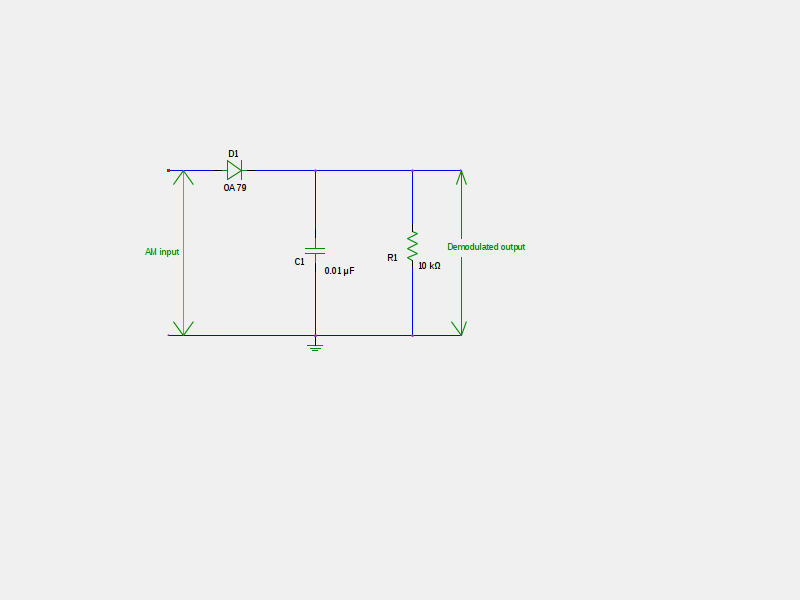
\includegraphics[width=15cm, height=10cm, trim=5cm 7.5cm 7.5cm 4cm, clip=true]{AMDemod.png}
\caption{AM Demodulation-Simple Diode Detector}
\label{AMDemod} 
\end{figure}
The circuit diagram for AM Demodulator using a simple diode detector is shown in Fig. \ref{AMDemod}.

\section*{Components and Equipments Required}
CRO, Function Generators(2), Breadboard, Probes.
\\Diodes- OA79
\\Capacitor- 0.01 $\mu$F
\\Resistor-10k$\Omega$
\section*{Procedure}

\begin{enumerate}
\item
Make connections on the breadboard as per the circuit diagram.
\item
Supply AM signal either from the signal generator or from the circuit designed in experiment Amplitude Modulation- Generation. 
\item
Connect the demodulated output to one channel of CRO along with the unmodulated signal on the other channel.
\item
Observe the Modulated and demodulated waveforms and plot it on a graph sheet.
\end{enumerate}
\section*{Observation}
A model plot showing the expected result of the experiment is shown in the Fig.\ref{AMdemod}
\begin{figure}
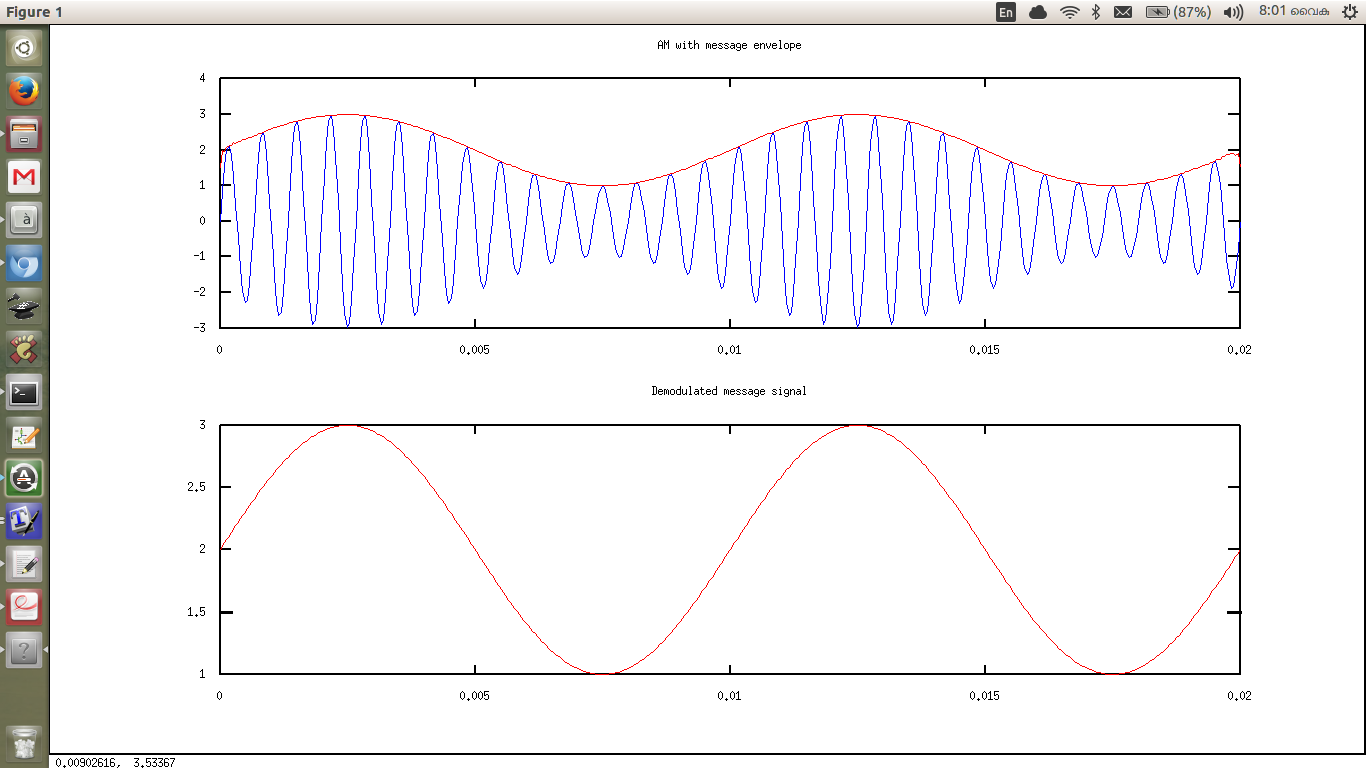
\includegraphics[width=12cm, height=10cm, trim= 2cm 1cm 1cm 1cm,clip=true]{AMdemod.png}
\caption{Modulated AM signal and Demodulated carrier}
\label{AMdemod}
\end{figure}

\section*{Result}

AM demodulation circuit was implemented on breadboard and output was observed and plotted ona graph sheet.
